\documentclass[english,xcolor=svgnames]{beamer}


\usepackage{mathptmx}
\usepackage[OT1]{fontenc}
% \usepackage[latin9]{inputenc}
\usepackage{amsmath}
\usepackage{amssymb}
\usepackage{amsthm}
\usepackage{mathrsfs}
\usepackage{amsfonts}
\usepackage{eurosym}
\usepackage{bm}

\usepackage{booktabs}
\usepackage{tabularx}
\usepackage{subcaption}
\usepackage[makeroom,thicklines]{cancel}

\usepackage{multirow}
\usepackage{rotating}
\usepackage{array}
\usepackage{float}



\makeatletter

 \newcommand\makebeamertitle{\frame{\maketitle}}%
 \AtBeginDocument{
   \let\origtableofcontents=\tableofcontents
 \def\tableofcontents{\@ifnextchar[{\origtableofcontents}{\gobbletableofcontents}}
   \def\gobbletableofcontents#1{\origtableofcontents}
 }
 
 \usetheme{Boadilla}
\setbeamertemplate{footline}[frame number]{}
\usefonttheme{structuresmallcapsserif}
\setbeamercolor{title}{fg=blue}
\setbeamercolor{frametitle}{fg=blue}
\setbeamercolor{caption name}{fg=blue}
\setbeamercovered{transparent}


\beamertemplatenavigationsymbolsempty

\usepackage{booktabs}
\usepackage{tabularx}
\renewcommand{\tabularxcolumn}[1]{>{\centering\arraybackslash}m{#1}}
%\newcolumntype{L}{>{\centering}X}
%\newcolumntype{H}{>{\lrbox0}c<{\endlrbox}@{}}

%\let\estinput=\input
%\newcommand{\estwide}[3]{
%          \vspace{.75ex}{
%               \begin{tabularx}
%               {\textwidth}{@{\hskip\tabcolsep\extracolsep\fill}l*{#2}{#3}}
%               \toprule
%               \estinput{#1}
%               \bottomrule
%               \addlinespace[.75ex]
%               \end{tabularx}
%               }
%          }
%
%		\newcommand{\figtext}[1]{
%		     %\vspace{-1.9ex}
%		     \captionsetup{justification=justified,font=footnotesize}
%		     \caption*{\hspace{6pt}\hangindent=1.5em #1}
%		     }
%		\newcommand{\fignote}[1]{\figtext{\emph{Note:~}~#1}}
%
\usepackage{collcell}
%\makeatother
% \newcolumntype{G}{>{\collectcell\@gobble}c<{\endcollectcell}@{}}
% \makeatother
% \def\eatcell#1\unskip{}
% \newcolumntype{E}{>{\eatcell}c@{}}
%\usepackage{tabulary}
%\usepackage{multirow}
%\usepackage{dcolumn}
%\usepackage{pdflscape}
%\usepackage{pdfpages}
% \usepackage{epsfig}
% \usepackage{epstopdf}
% \usepackage{eso-pic}
\usepackage{graphicx}
%\usepackage{arydshln}
\usepackage[compatibility=false,font={sc,rm,color=blue},justification=centering,labelformat=empty, textfont=Large, margin=2pt]{caption}
\captionsetup[figure]{belowskip=0pt}

\newcommand{\rot}[2]{\rule{1em}{0pt}%
\makebox[0cm][c]{\rotatebox{#1}{\ #2}}}

\usepackage{siunitx} %For aligning decimals
\sisetup{ detect-mode, 
          group-digits            = false ,
          input-signs             = ,
          input-symbols           = ()[]-+* ,
          input-open-uncertainty  = ,
          input-close-uncertainty = ,
          table-align-text-post   = false, 
          table-number-alignment = center
}
\selectcolormodel{cmyk}
\usepackage{color,soul}
\usepackage{colortbl}
\usepackage{tikz}
\usetikzlibrary{matrix,shapes,arrows,intersections,calc}
\usepackage{verbatim}
\setbeamercovered{invisible}
\setbeamercolor{math text displayed}{fg=blue}
\setbeamercolor{math text inlined}{fg=blue}

%\let\olditem\item
%\renewcommand{\item}{\setlength{\itemsep}{\fill}\olditem}
\AtBeginDocument{\setlength\belowdisplayskip{0pt}}


\usepackage[english]{babel}
\usepackage{booktabs}
\usepackage{tablefootnote}
\usepackage{calc,hhline,ifthen,lscape} 

%\usepackage{enumitem}
%\let\olditem\item
%\renewcommand{\item}{\setlength{\itemsep}{\fill}\olditem}

% new math commands
\newcommand{\E}{\mathbb{E}}

\newcommand{\sym}[1]{\rlap{$#1$}} %For sym in STATA tables

\setbeamertemplate{frametitle}[default][center]

% \makeglossaries
% 
% \usepackage{pgfpages}
% \pgfpagesuselayout{resize to}[a4paper, landscape, border shrink=5mm]
\usepackage[absolute,overlay]{textpos}

\usepackage{epstopdf}


%\setlength{\itemsep}{\fill}



% ===========================================================
% ===========================================================
% ===========================================================
% Improves spacing of itemize and enumerate environment

\makeatletter
\renewcommand{\itemize}[1][]{%
  \beamer@ifempty{#1}{}{\def\beamer@defaultospec{#1}}%
  \ifnum \@itemdepth >2\relax\@toodeep\else
    \advance\@itemdepth\@ne
    \beamer@computepref\@itemdepth% sets \beameritemnestingprefix
    \usebeamerfont{itemize/enumerate \beameritemnestingprefix body}%
    \usebeamercolor[fg]{itemize/enumerate \beameritemnestingprefix body}%
    \usebeamertemplate{itemize/enumerate \beameritemnestingprefix body begin}%
    \list
      {\usebeamertemplate{itemize \beameritemnestingprefix item}}
      {\def\makelabel##1{%
          {%
            \hss\llap{{%
                \usebeamerfont*{itemize \beameritemnestingprefix item}%
                \usebeamercolor[fg]{itemize \beameritemnestingprefix item}##1}}%
          }%
        }%
      }
  \fi%
  \setlength\itemsep{\fill}
    \ifnum \@itemdepth >1
        \vfill
    \fi%  
  \beamer@cramped%
  \raggedright%
  \beamer@firstlineitemizeunskip%
}

\def\enditemize{\ifhmode\unskip\fi\endlist%
  \usebeamertemplate{itemize/enumerate \beameritemnestingprefix body end}
  \ifnum \@itemdepth >1
        \vfil
  \fi%  
  }
\makeatother


\makeatletter
\def\enumerate{%
	\ifnum\@enumdepth>2\relax\@toodeep
	\else%
	\advance\@enumdepth\@ne%
	\edef\@enumctr{enum\romannumeral\the\@enumdepth}%
	\advance\@itemdepth\@ne%
	\fi%
	\beamer@computepref\@enumdepth% sets \beameritemnestingprefix
	\edef\beamer@enumtempl{enumerate \beameritemnestingprefix item}%
	\@ifnextchar[{\beamer@@enum@}{\beamer@enum@}}
\def\beamer@@enum@[{\@ifnextchar<{\beamer@enumdefault[}{\beamer@@@enum@[}}
\def\beamer@enumdefault[#1]{\def\beamer@defaultospec{#1}%
	\@ifnextchar[{\beamer@@@enum@}{\beamer@enum@}}
\def\beamer@@@enum@[#1]{% partly copied from enumerate.sty
	\@enLab{}\let\@enThe\@enQmark
	\@enloop#1\@enum@
	\ifx\@enThe\@enQmark\@warning{The counter will not be printed.%
		^^J\space\@spaces\@spaces\@spaces The label is: \the\@enLab}\fi
	\def\insertenumlabel{\the\@enLab}
	\def\beamer@enumtempl{enumerate mini template}%
	\expandafter\let\csname the\@enumctr\endcsname\@enThe
	\csname c@\@enumctr\endcsname7
	\expandafter\settowidth
	\csname leftmargin\romannumeral\@enumdepth\endcsname
	{\the\@enLab\hspace{\labelsep}}%
	\beamer@enum@}
\def\beamer@enum@{%
	\beamer@computepref\@itemdepth% sets \beameritemnestingprefix
	\usebeamerfont{itemize/enumerate \beameritemnestingprefix body}%
	\usebeamercolor[fg]{itemize/enumerate \beameritemnestingprefix body}%
	\usebeamertemplate{itemize/enumerate \beameritemnestingprefix body begin}%
	\expandafter
	\list
	{\usebeamertemplate{\beamer@enumtempl}}
	{\usecounter\@enumctr%
		\def\makelabel##1{{\hss\llap{{%
						\usebeamerfont*{enumerate \beameritemnestingprefix item}%
						\usebeamercolor[fg]{enumerate \beameritemnestingprefix item}##1}}}}}%
	\setlength\itemsep{\fill}
	\ifnum \@itemdepth >1
	\vfill
	\fi%  
	\beamer@cramped%
	\raggedright%
	\beamer@firstlineitemizeunskip%
}
\def\endenumerate{\ifhmode\unskip\fi\endlist%
	\usebeamertemplate{itemize/enumerate \beameritemnestingprefix body end}
	\ifnum \@itemdepth >1
	\vfil
	\fi%  
}
\makeatother

% ===========================================================
% ===========================================================
% ===========================================================


%\usepackage[colorlinks=true]{hyperref}

\hypersetup{colorlinks = true,linkcolor = blue, bookmarksopen=true, bookmarksopenlevel=1}

%\hypersetup{bookmarksopen=true, bookmarksopenlevel=1}



\begin{document}

\title{Macroeconomics of Consumption with Heterogeneity}
\vspace{1cm}
\author[shortname]{
\begin{tabular}{cc}
Juan Herre\~{n}o & Johannes Wieland \\ 
\end{tabular}\\
}



\date{UCSD, Spring \the\year}

\setbeamertemplate{footline}{}
\makebeamertitle
\setbeamertemplate{footline}[frame number]{}

\addtocounter{framenumber}{-1}



%\begin{frame}
%\frametitle[alignment=center]{Reminders}
%\begin{enumerate}
%	\item First project draft due May 1.
%	\item Participation.
%\end{enumerate}
%\end{frame}


%%%%%%%%%%%%%%%%%%%%%%%%%%%%%%%%%%%%%%%%%%%%%%%%%%
\AtBeginSection[]{
\setbeamertemplate{footline}{}
  \frame<beamer>{ 

    \frametitle{Outline}   

    \tableofcontents[currentsection,hideallsubsections] 
  }
\setbeamertemplate{footline}[frame number]{}
\addtocounter{framenumber}{-1}
}

\AtBeginSubsection[]{
\setbeamertemplate{footline}{}
  \frame<beamer>{ 

    \frametitle{Outline}   

    \tableofcontents[currentsection,currentsubsection] 
  }
  \setbeamertemplate{footline}[frame number]{}
  \addtocounter{framenumber}{-1}
}



\setbeamertemplate{footline}{}
\begin{frame}
\frametitle{Outline}   
\tableofcontents[hideallsubsections] 
\end{frame}
\addtocounter{framenumber}{-1}
\setbeamertemplate{footline}[frame number]{}


%%%%%%%%%%%%%%%%%%%%%%%%%%%%%%%%%%%%%%%%%%%%%%%%%%
\section{Introduction}
%%%%%%%%%%%%%%%%%%%%%%%%%%%%%%%%%%%%%%%%%%%%%%%%%%



%%%%%%%%%%%%%%%%%%%%%%%%%%%%%%%%%%%%%%%%%%%%%%%%%%
\section{Auclert, Rognlie, Straub (2020)}
%%%%%%%%%%%%%%%%%%%%%%%%%%%%%%%%%%%%%%%%%%%%%%%%%%

\begin{frame}
    \frametitle{New Keynesian Model in Sequence Space}
    \begin{itemize}
        \item Consumption function:
        \begin{align*}
            C_t &= \mathbb{C}(\{Y_{t+s}-T_{t+s},r_{t+s}\}_{s=0}^{\infty}) \\
            &\equiv \mathbb{C}(\bm{Y}-\bm{T},\bm{r})
        \end{align*}
        \item NKPC:
        \begin{align*}
            \pi_t &= \mathbb{S}(\bm{Y} - \bm{Y}^*) 
        \end{align*}
        \item Interest rate rule:
        \begin{align*}
            \bm{r} &= \bm{\Phi}_Y (\bm{Y} - \bm{Y}^*) +  \bm{\Phi}_\pi \bm{\pi} + \bm{\epsilon}^r 
        \end{align*}
        \item Excess demand:
        \begin{align*}
%            \begin{pmatrix} ED_t \\ ED_{t+1} \\ \vdots \end{pmatrix}= 
            \bm{ED} &= \pmb{\mathbb{C}}(\bm{Y}-\bm{T},\bm{r}) + \bm{G} - \bm{Y} =\bm{0}
        \end{align*}
%        \item In equilibrium, $\bm{ED}=\bm{0}$.
    \end{itemize}
\end{frame}

\begin{frame}
    \frametitle{Linearize to Solve with Linear Algebra}
    \begin{itemize}
        \item Linearized Model:
        \begin{align*}
            \bm{\hat{C}} &= (\nabla_{\bm{Y}}\pmb{\mathbb{C}}) (\bm{\hat{Y}} - \bm{\hat{T}}) + (\nabla_{\bm{r}}\pmb{\mathbb{C}})\bm{\hat{r}} \\
            \bm{\hat{\pi}} &= (\nabla_{\bm{Y}}\pmb{\mathbb{S}})(\bm{\hat{Y}} - \bm{\hat{Y}}^*)  \\
            \bm{\hat{r}} &= \bm{\Phi}_Y (\bm{\hat{Y}} - \bm{\hat{Y}}^*) +  \bm{\Phi}_\pi \bm{\hat{\pi}} + \bm{\epsilon}^r 
        \end{align*}
        \item Equilibrium:
         \begin{align*}
             \bm{\hat{Y}} &=  [ \bm{\Phi}_Y  +  \bm{\Phi}_\pi (\nabla_{\bm{Y}}\pmb{\mathbb{S}}) ]^{-1} \{[ \bm{\Phi}_Y  +  \bm{\Phi}_\pi (\nabla_{\bm{Y}}\pmb{\mathbb{S}}) ]^{-1} - [I - \nabla_{\bm{Y}}\pmb{\mathbb{C}}]^{-1}(\nabla_{\bm{r}}\pmb{\mathbb{C}})  \}^{-1}  \times\\ 
             &\times[I - \nabla_{\bm{Y}}\pmb{\mathbb{C}}]^{-1} [\bm{\hat{G}} - (\nabla_{\bm{Y}}\pmb{\mathbb{C}})\bm{\hat{T}} + (\nabla_{\bm{r}}\pmb{\mathbb{C}})\bm{\epsilon}^r ]  
         \end{align*}
         \item Kaplan, Moll, and Violante (2018):
         \begin{itemize}
         	\item Small direct effect $\nabla_{\bm{r}}\pmb{\mathbb{C}}$
         	\item Large indirect effect $[I - \nabla_{\bm{Y}}\pmb{\mathbb{C}}]^{-1}$
         	\item Product roughly constant $[I - \nabla_{\bm{Y}}\pmb{\mathbb{C}}]^{-1}(\nabla_{\bm{r}}\pmb{\mathbb{C}})$
         \end{itemize}
         \item[$\Rightarrow$] Should we care about the decomposition?
    \end{itemize}
\end{frame}


\begin{frame}
    \frametitle{Add Investment}
    \begin{itemize}
        \item Yes:
        \begin{align*}
             \bm{\hat{Y}} &=  [ \bm{\Phi}_Y  +  \bm{\Phi}_\pi (\nabla_{\bm{Y}}\pmb{\mathbb{S}}) ]^{-1} \times \\
             &\times \{[ \bm{\Phi}_Y  +  \bm{\Phi}_\pi (\nabla_{\bm{Y}}\pmb{\mathbb{S}}) ]^{-1} - [I - \nabla_{\bm{Y}}\pmb{\mathbb{C}} - \nabla_{\bm{Y}}\pmb{\mathbb{I}} ]^{-1}(\nabla_{\bm{r}}\pmb{\mathbb{C}} + \nabla_{\bm{r}}\pmb{\mathbb{I}})  \}^{-1}  \times\\ 
             &\times[I - \nabla_{\bm{Y}}\pmb{\mathbb{C}}- \nabla_{\bm{Y}}\pmb{\mathbb{I}}]^{-1} [\bm{\hat{G}} - (\nabla_{\bm{Y}}\pmb{\mathbb{C}})\bm{\hat{T}} + (\nabla_{\bm{r}}\pmb{\mathbb{C}}+\nabla_{\bm{r}}\pmb{\mathbb{I}})\bm{\epsilon}^r ]  
         \end{align*}
        \item Key challenge: How to set up model to match 
        \begin{itemize}
        	\item Immediate consumption response to higher income (``jump'').
        	\item Delayed consumption, investment, output response to lower real interest rate (``hump'').
        \end{itemize}
    \end{itemize}
\end{frame}


\begin{frame}
    \frametitle{The Challenge}
    \begin{center}
    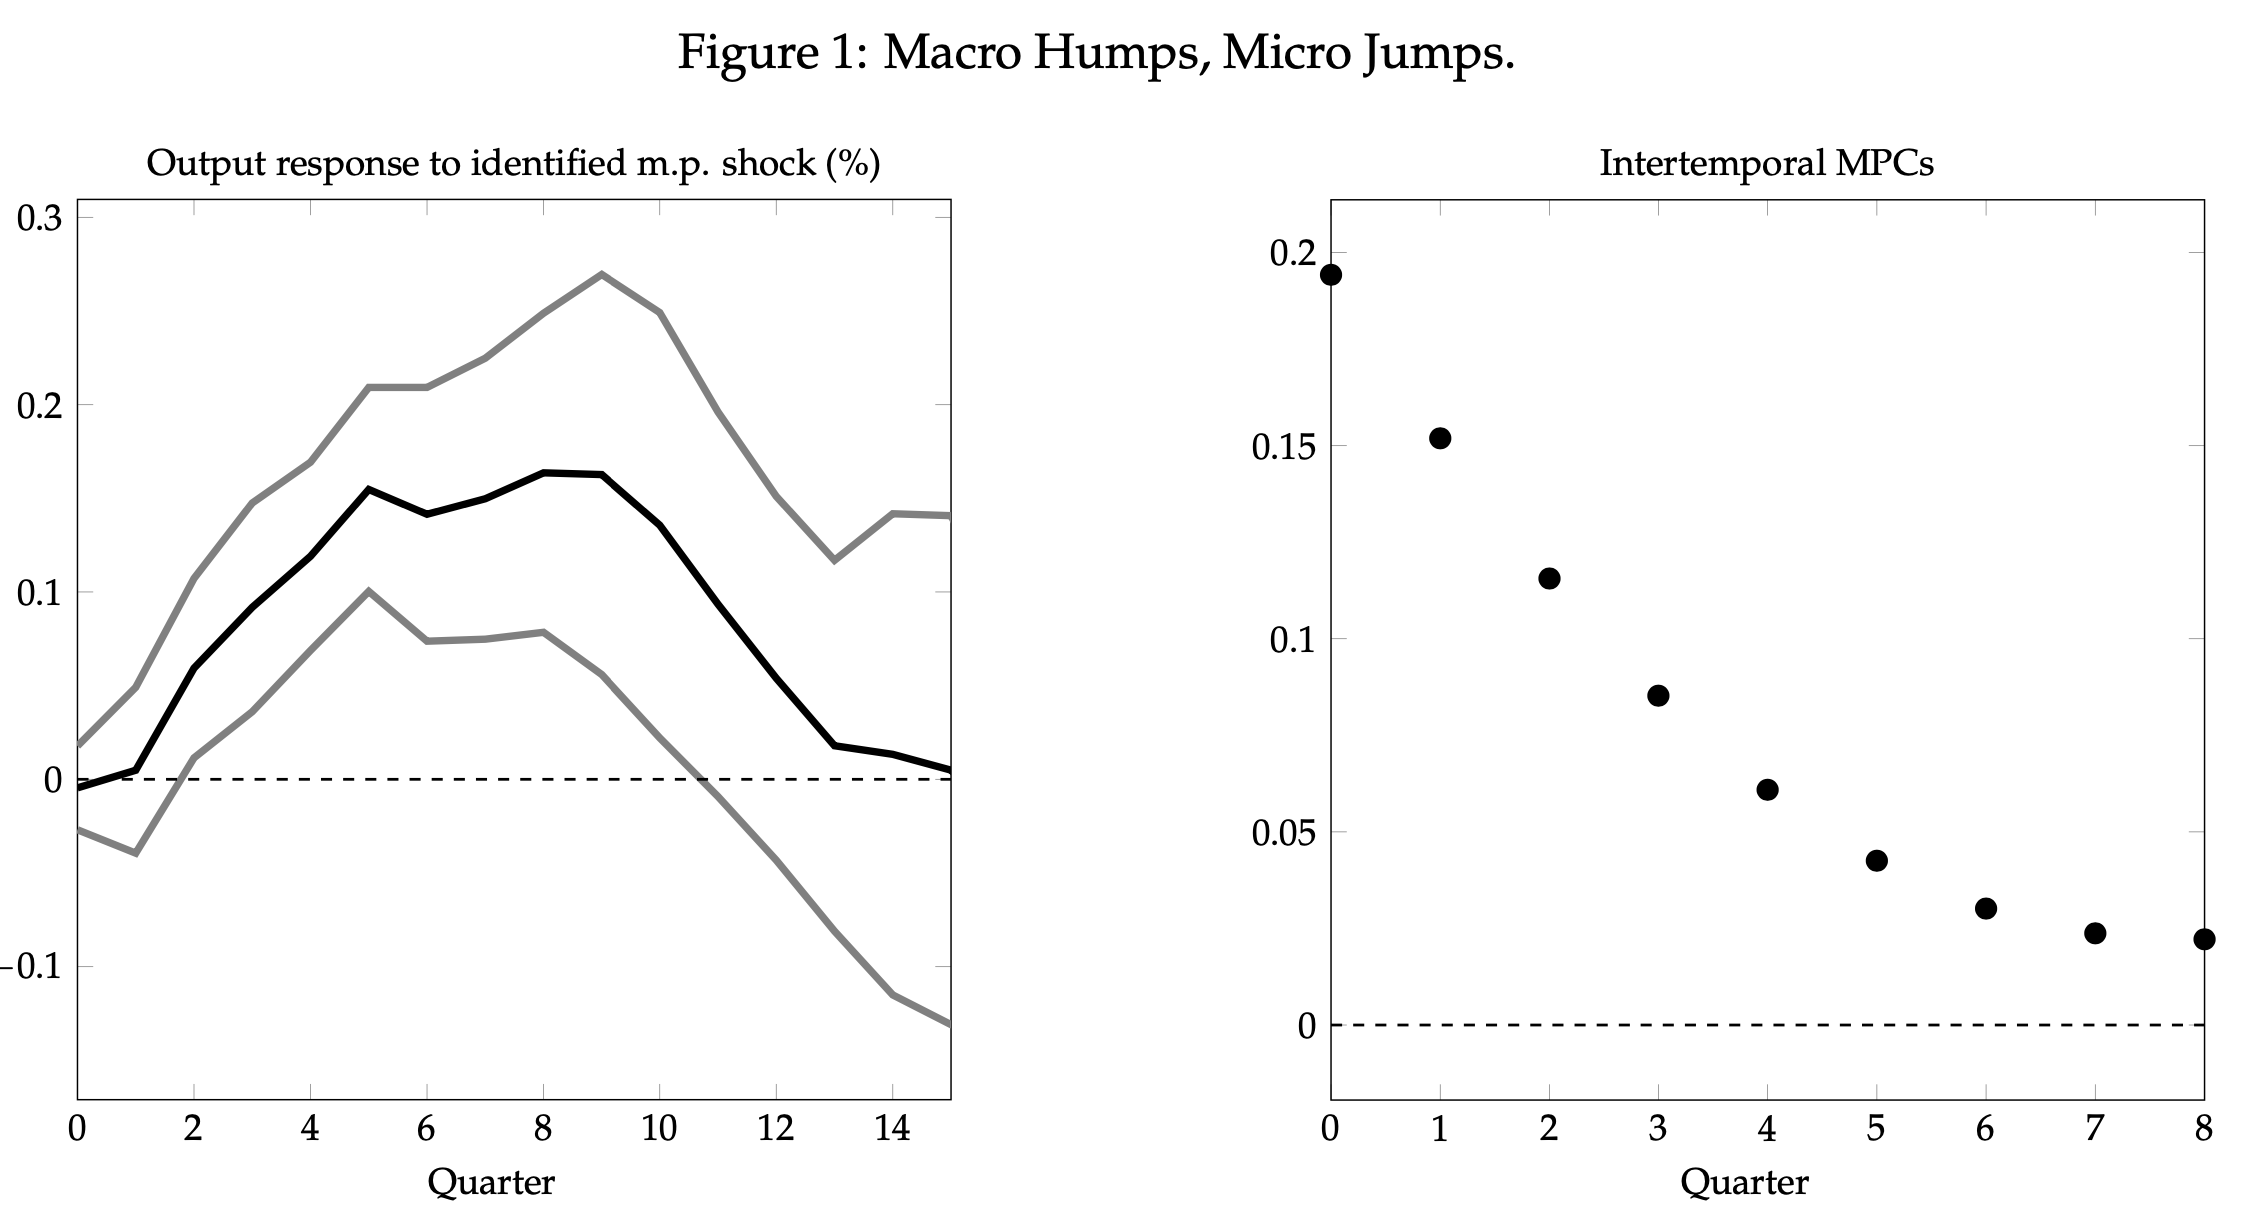
\includegraphics[scale=0.3]{figures/ARSFIG1.png}
    \end{center}
\end{frame}

\begin{frame}
    \frametitle{Model}
    \begin{itemize}
        \item Household problem:
        \begin{align*}
        	V_t(l,s) = &\max_{c,l'}u(c)+\beta\E[V_{t+1}(l',s')|s] \\
        	&c'+l' \le (1+r_t)l + y_t e(s) \\
        	& l'\ge 0
        \end{align*}
        \item Standard sequence space result:
        \begin{align*}
        	C_t = \mathcal{C}(\{y_s,r_s\}_{s\ge 0}), \;t\ge 0
        \end{align*}
    \end{itemize}
\end{frame}

\begin{frame}
    \frametitle{Matching Micro Data}
    \begin{center}
    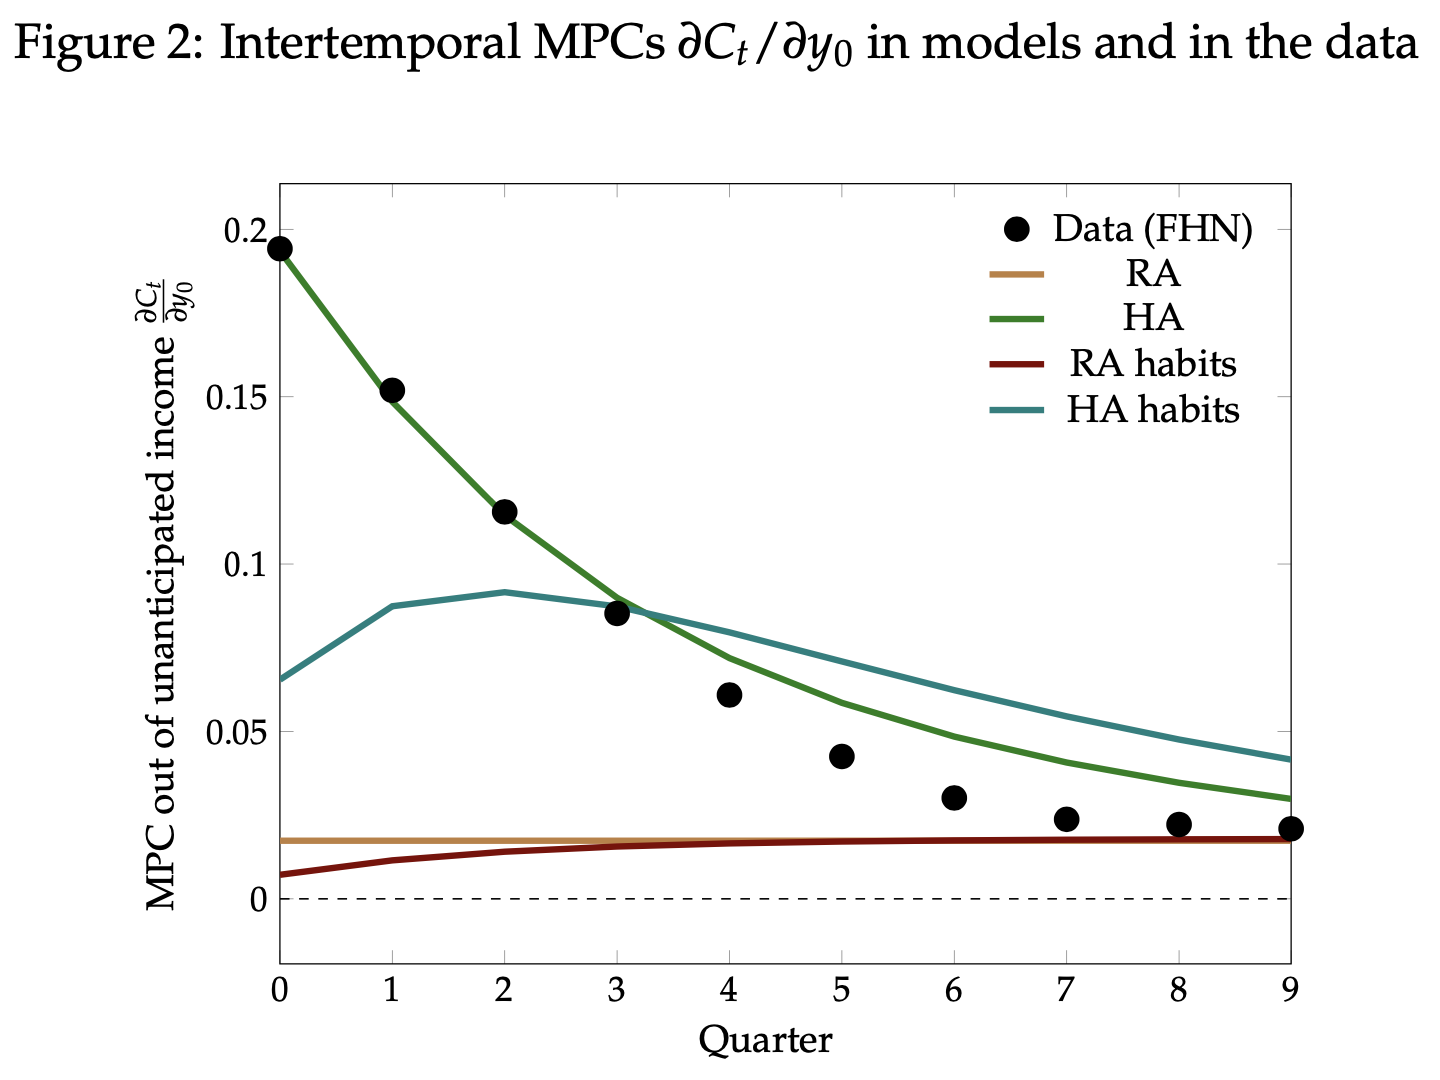
\includegraphics[scale=0.4]{figures/ARSFIG2.png}
    \end{center}
    \begin{itemize}
    	\item Why does habit model have difficulty?
    \end{itemize}
\end{frame}

\begin{frame}
    \frametitle{Inattention}
    \begin{itemize}
        \item Households know current micro state $e(s)$.
        \item Households update info about aggregate shocks with iid probability $1-\theta$ each period.
        \item Households know current $r_t,Y_t$ but forecast $r_{t+s},Y_{t+s}$ using info from $t-k$. 
        \item[$\Rightarrow$] Households always on budget constraint.
        \item Optimize subject to information from $k$ periods ago:
        \begin{align*}
        	V_t(l,s,k) = &\max_{c,l'}u(c)+\beta\E_{t-k}[\theta V_{t+1}(l',s',k+1) + (1-\theta) V_{t+1}(l',s',0)|s] 
        \end{align*}
    \end{itemize}
\end{frame}

\begin{frame}
    \frametitle{Estimation}
    \begin{itemize}
        \item Two-step procedure.
        \item Calibrate household problem to micro data, so only need to compute household sequence space Jacobians once.
        \item Estimate information and macro parameters to match estimated IRF to monetary policy shocks.
        \item Sticky info micro Jacobian at $t$ to shock at time $s$:
        \begin{align*}
        	\mathcal{J}_{t,s}^{o,i} = \begin{cases}
        		\theta\mathcal{J}_{t-1,s-1}^{o,i} + (1-\theta)\mathcal{J}_{t,s}^{o,i,FI} & t>0, s>0 \\
        		\mathcal{J}_{t,s}^{o,i,FI} & s=0 \\
        		(1-\theta)\mathcal{J}_{t,s}^{o,i,FI} & t=0, s>0
        	\end{cases}
        \end{align*}
    \end{itemize}
\end{frame}




\begin{frame}
    \frametitle{Calibration}
    \begin{center}
    	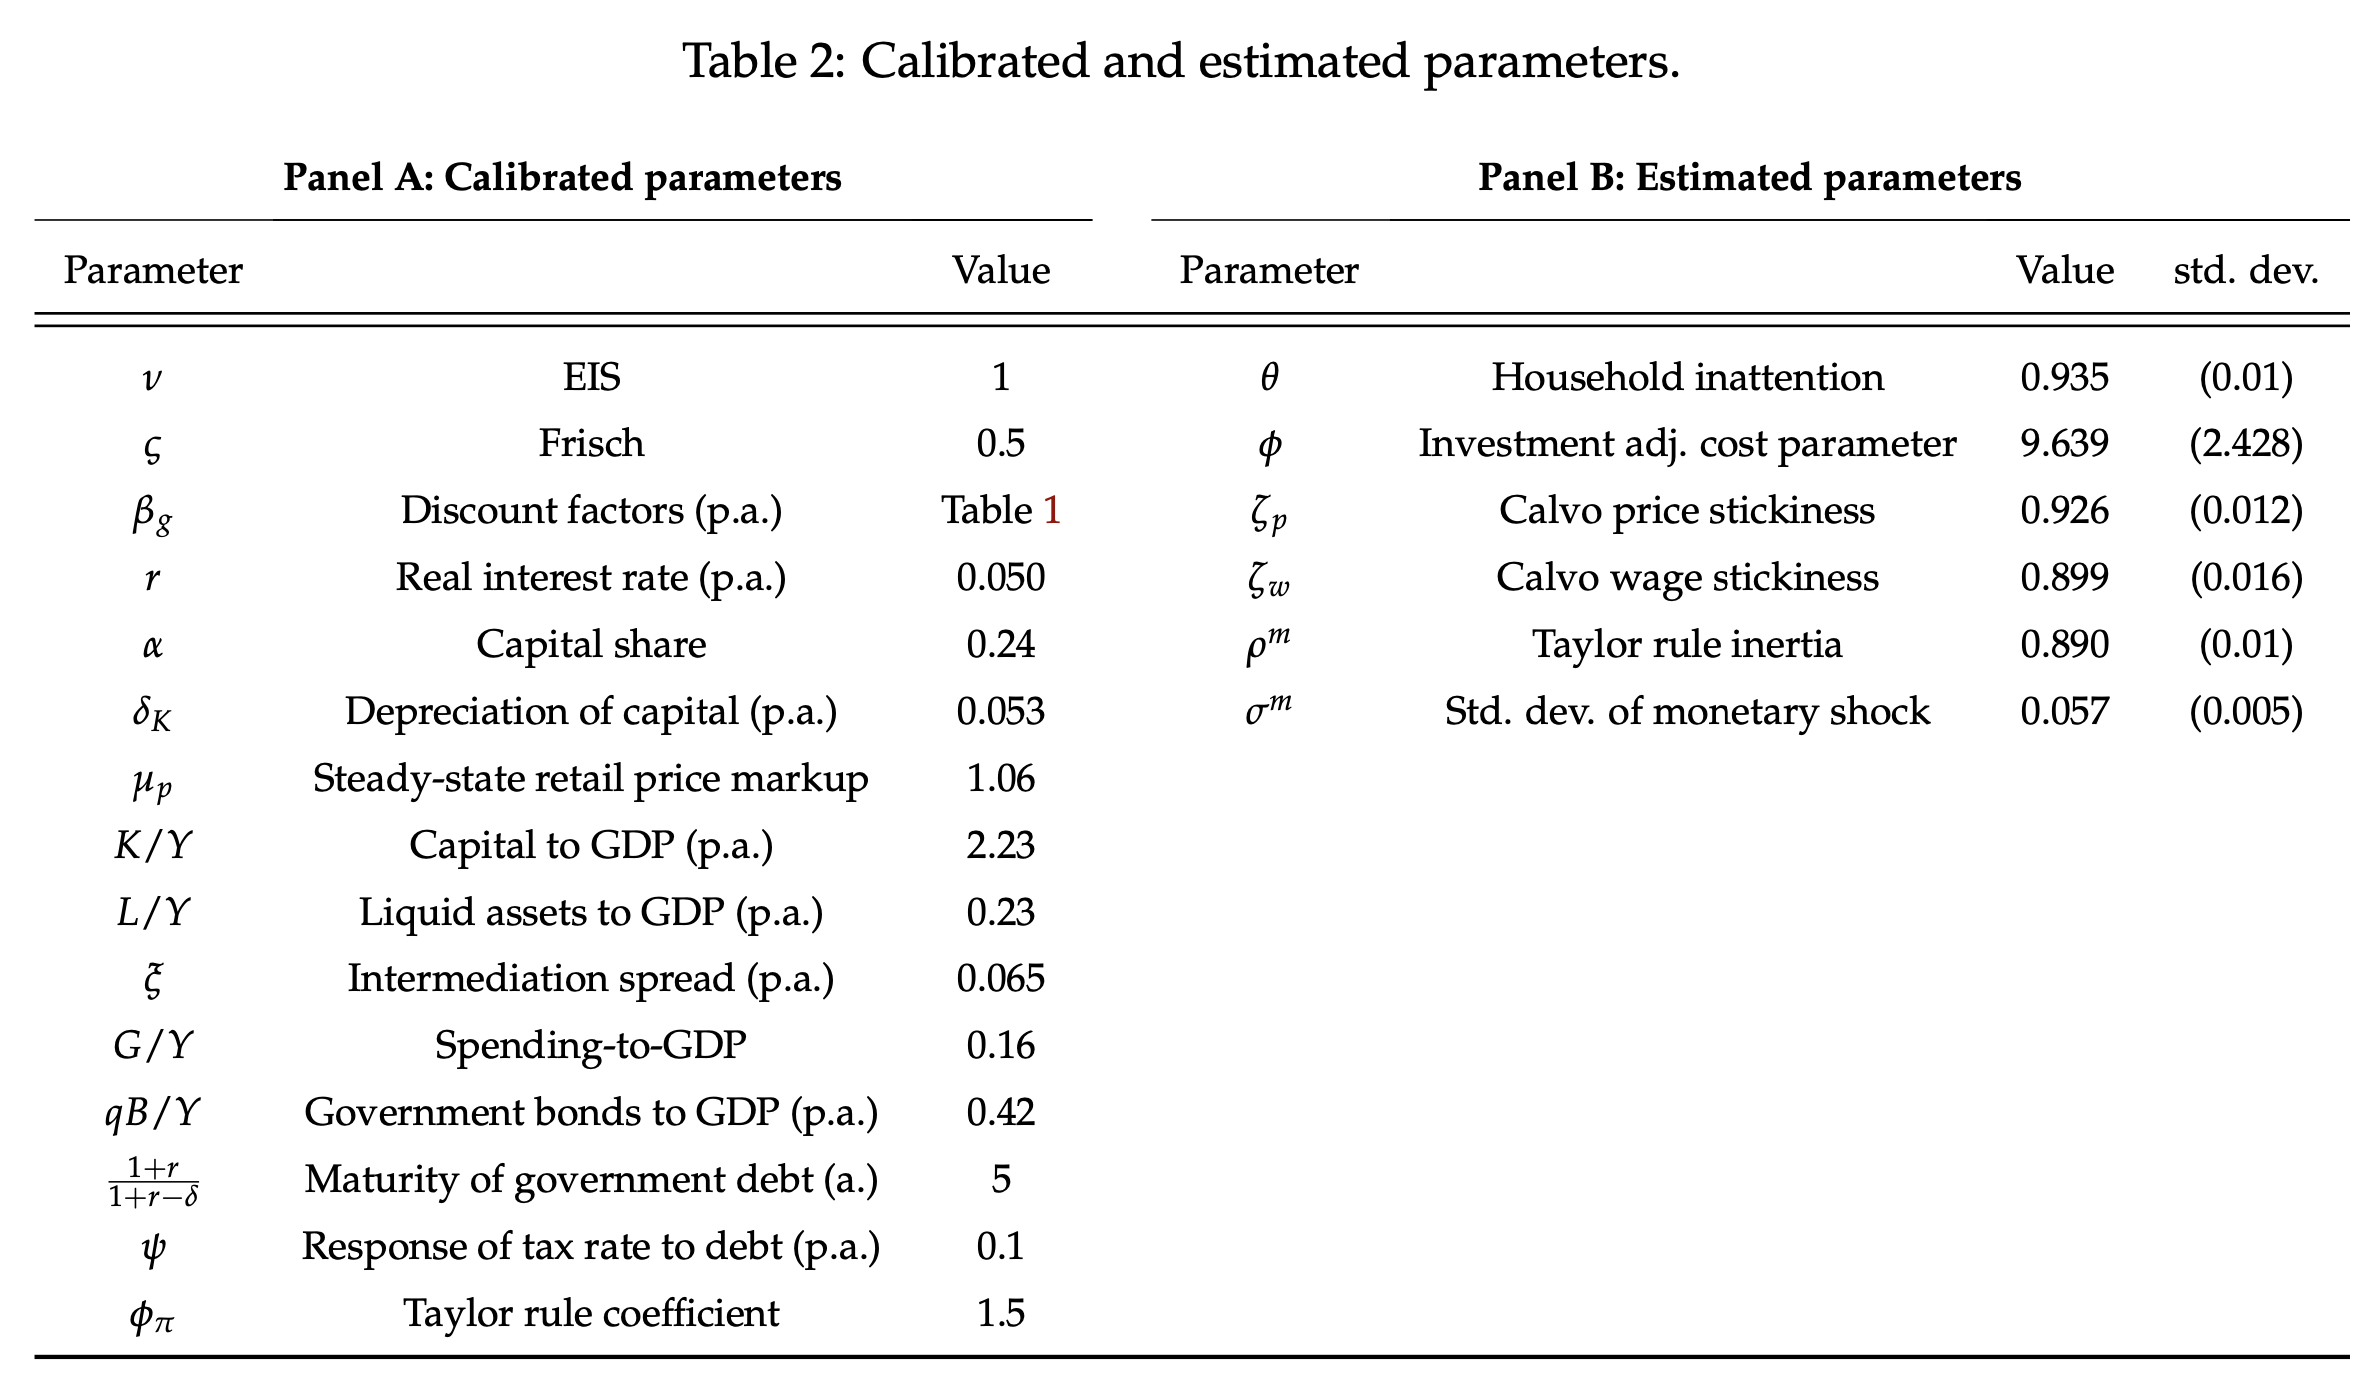
\includegraphics[scale=0.25]{figures/ARSTAB2.png}	
    \end{center}
\end{frame}


\begin{frame}
    \frametitle{Matching the Humps}
    \begin{center}
    	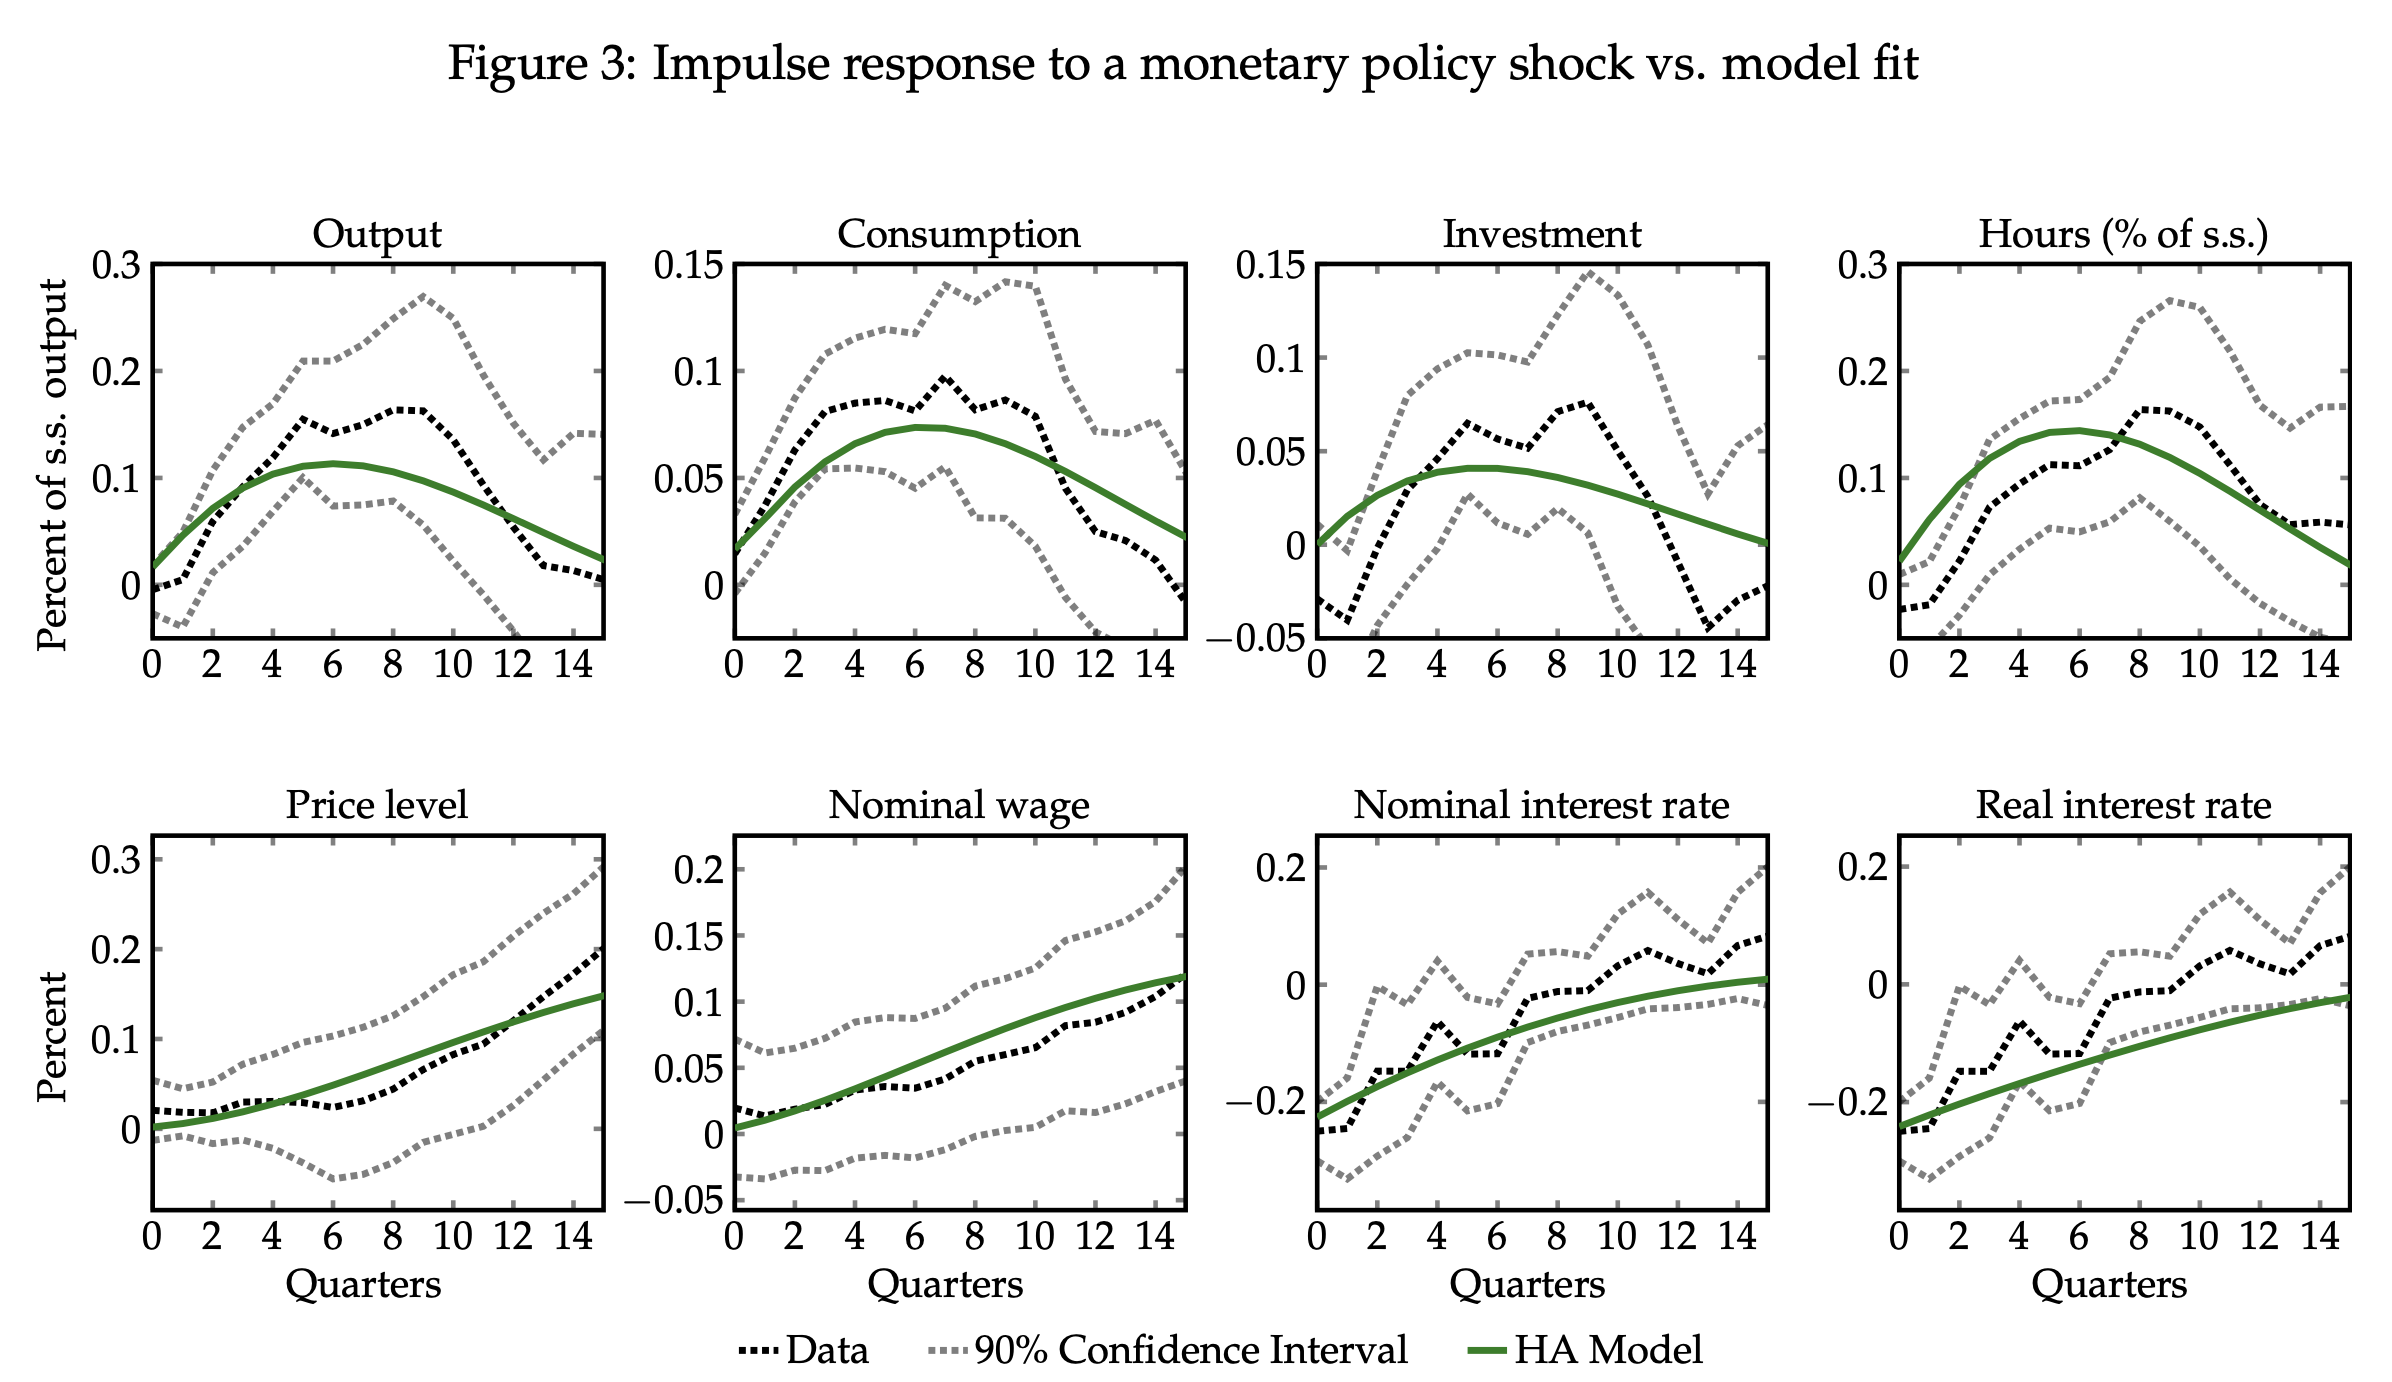
\includegraphics[scale=0.25]{figures/ARSFIG3.png}	
    \end{center}
\end{frame}

\begin{frame}
    \frametitle{Role of Inattention}
    \begin{center}
    	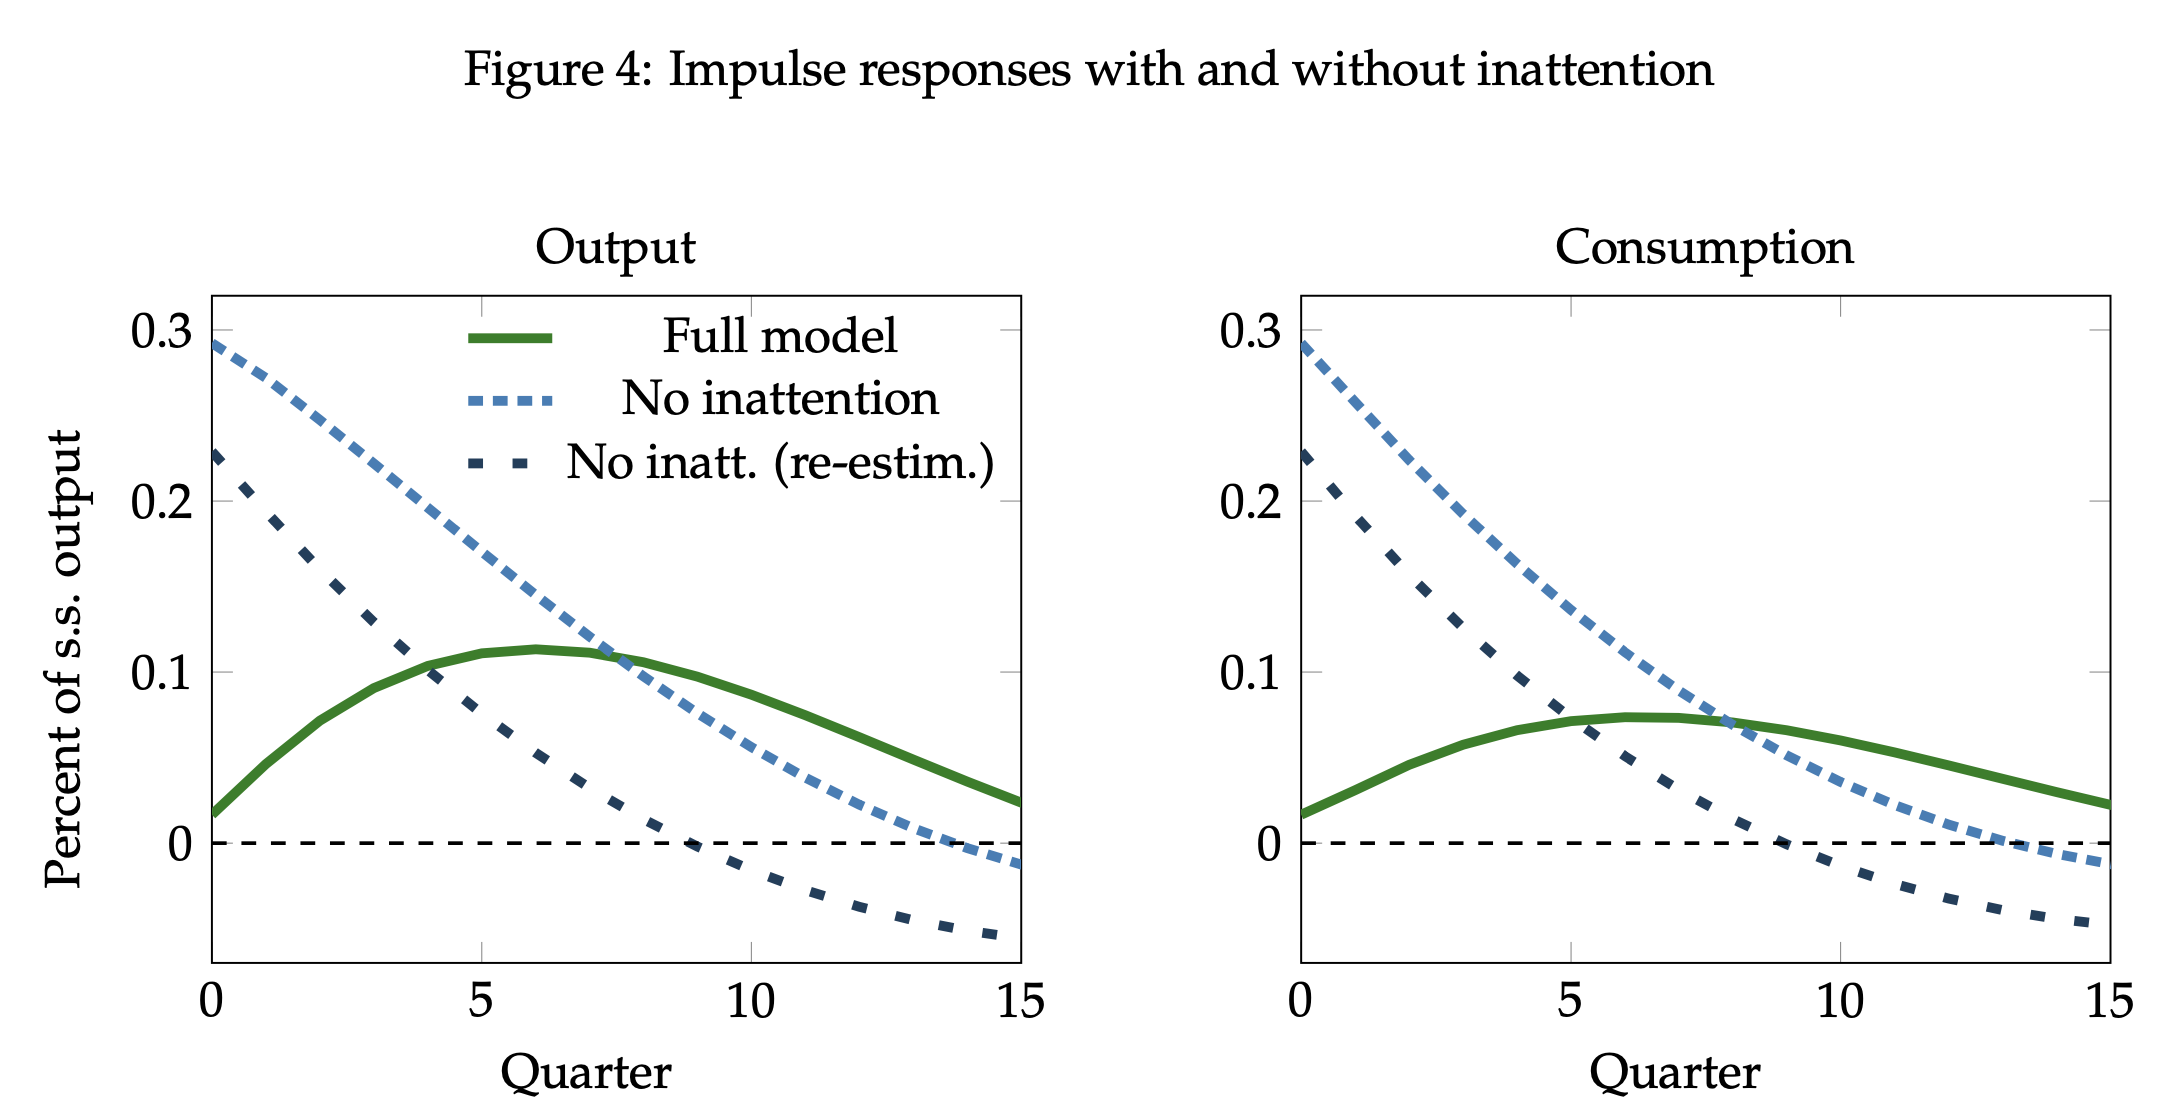
\includegraphics[scale=0.3]{figures/ARSFIG4.png}	
    \end{center}
\end{frame}


\begin{frame}
    \frametitle{Importance of Investment}
    \begin{center}
    	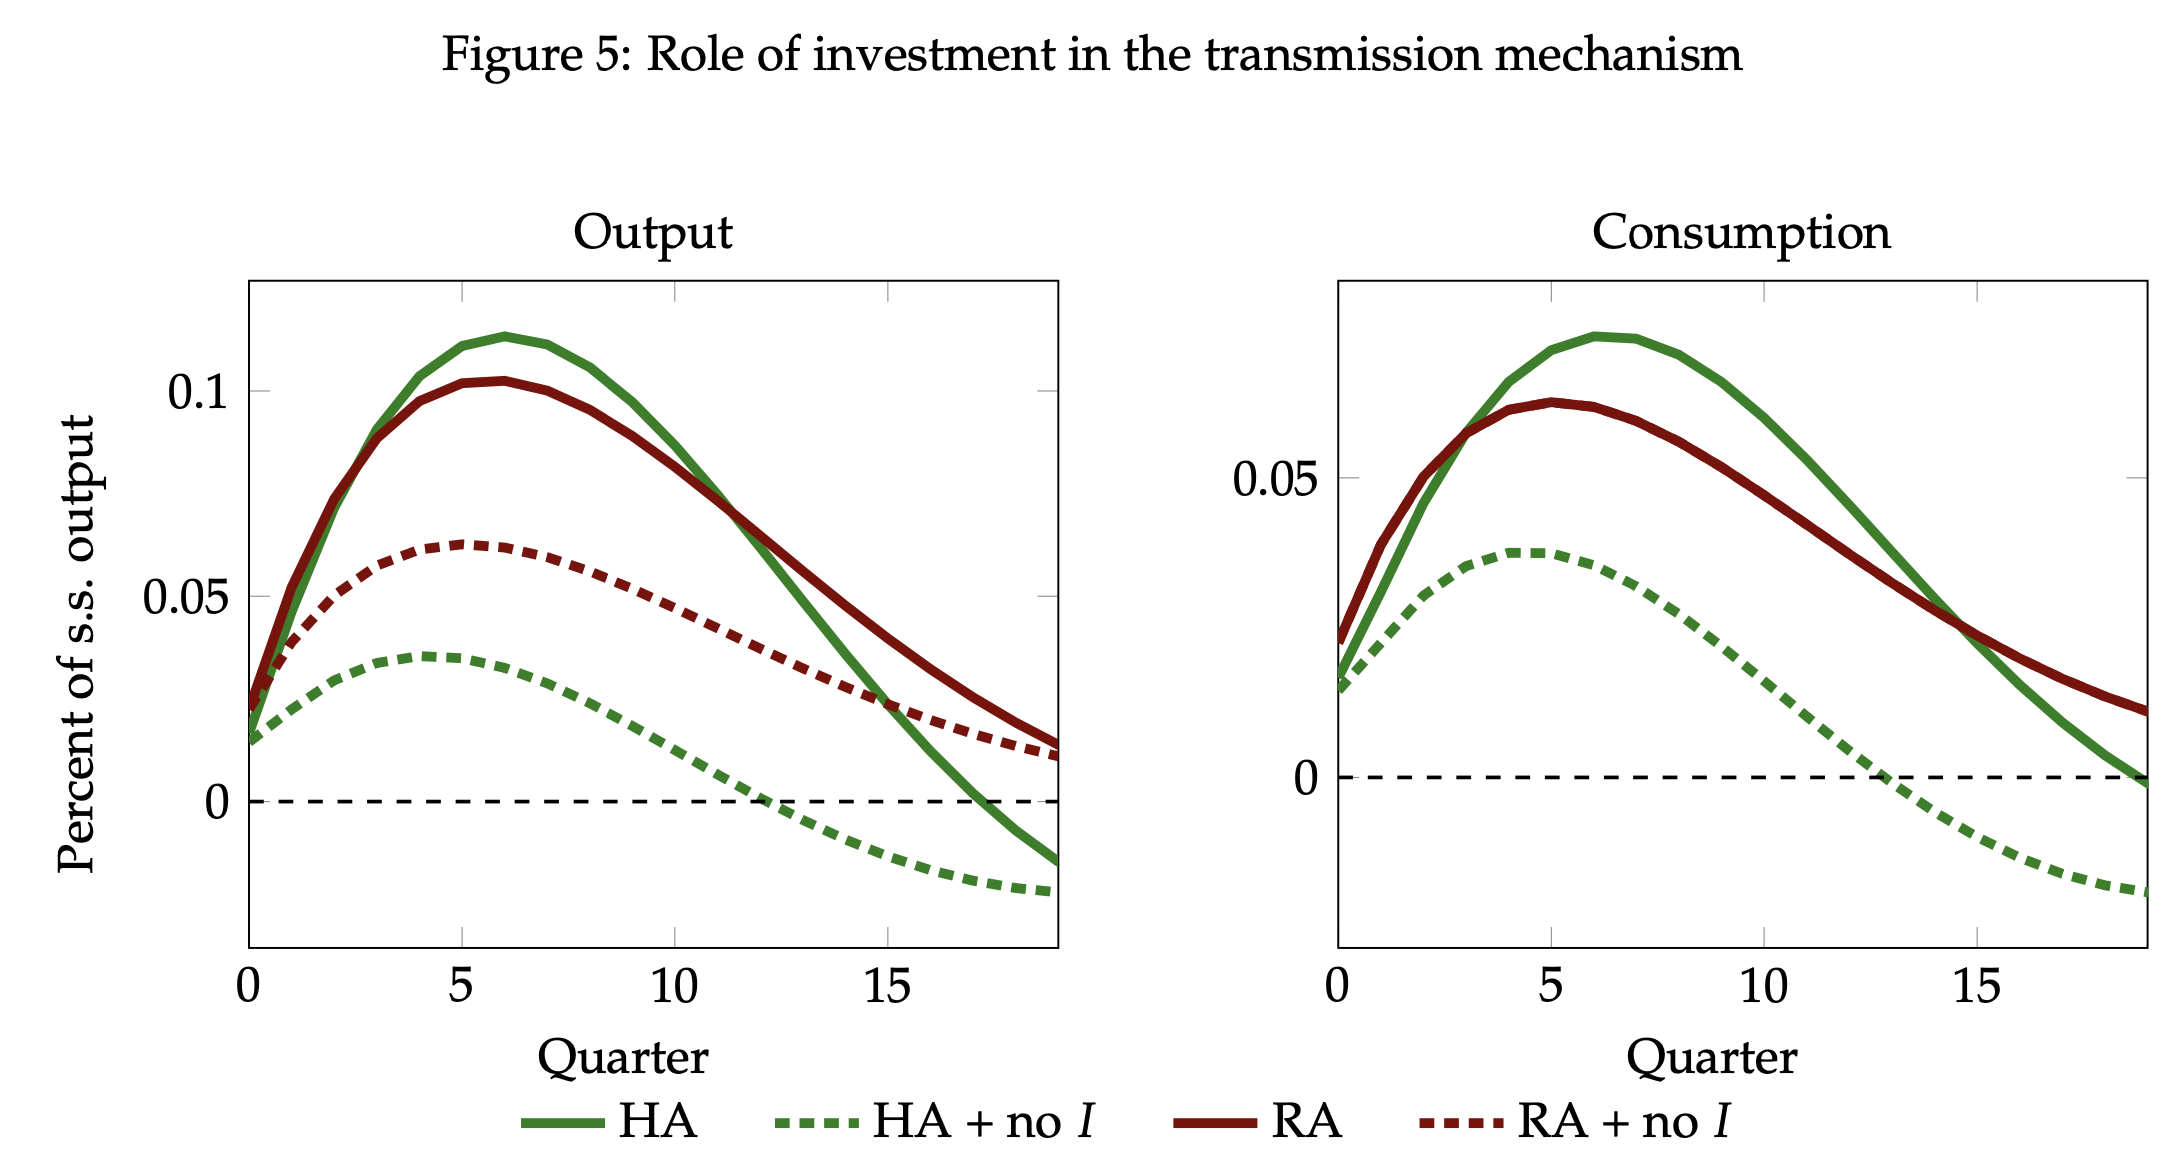
\includegraphics[scale=0.3]{figures/ARSFIG5.png}	
    \end{center}
\end{frame}

\begin{frame}
    \frametitle{Direct vs Indirect Effects}
    \begin{center}
    	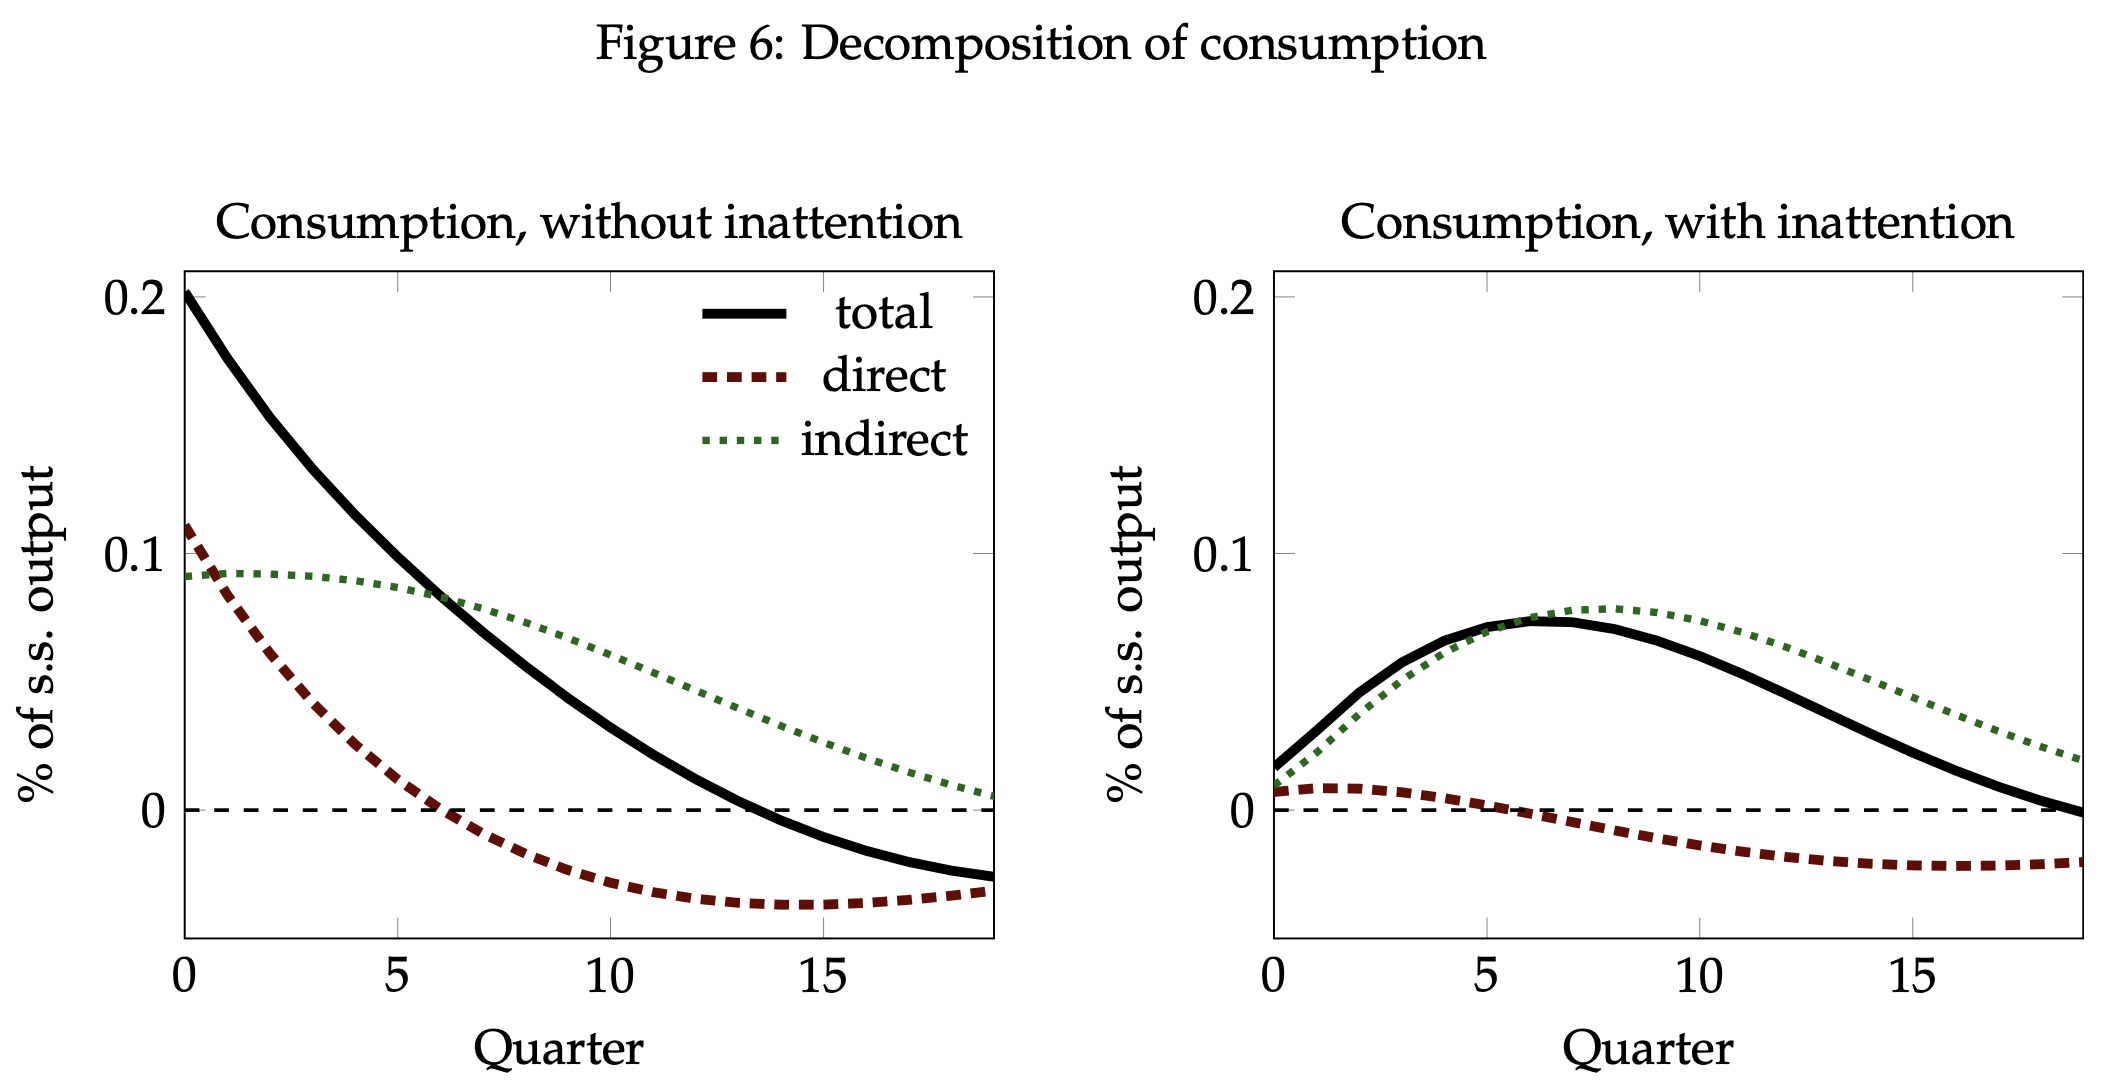
\includegraphics[scale=0.3]{figures/ARSFIG6.png}	
    \end{center}
\end{frame}

\begin{frame}
    \frametitle{Aside: Role of Fiscal Policy}
    \begin{center}
    	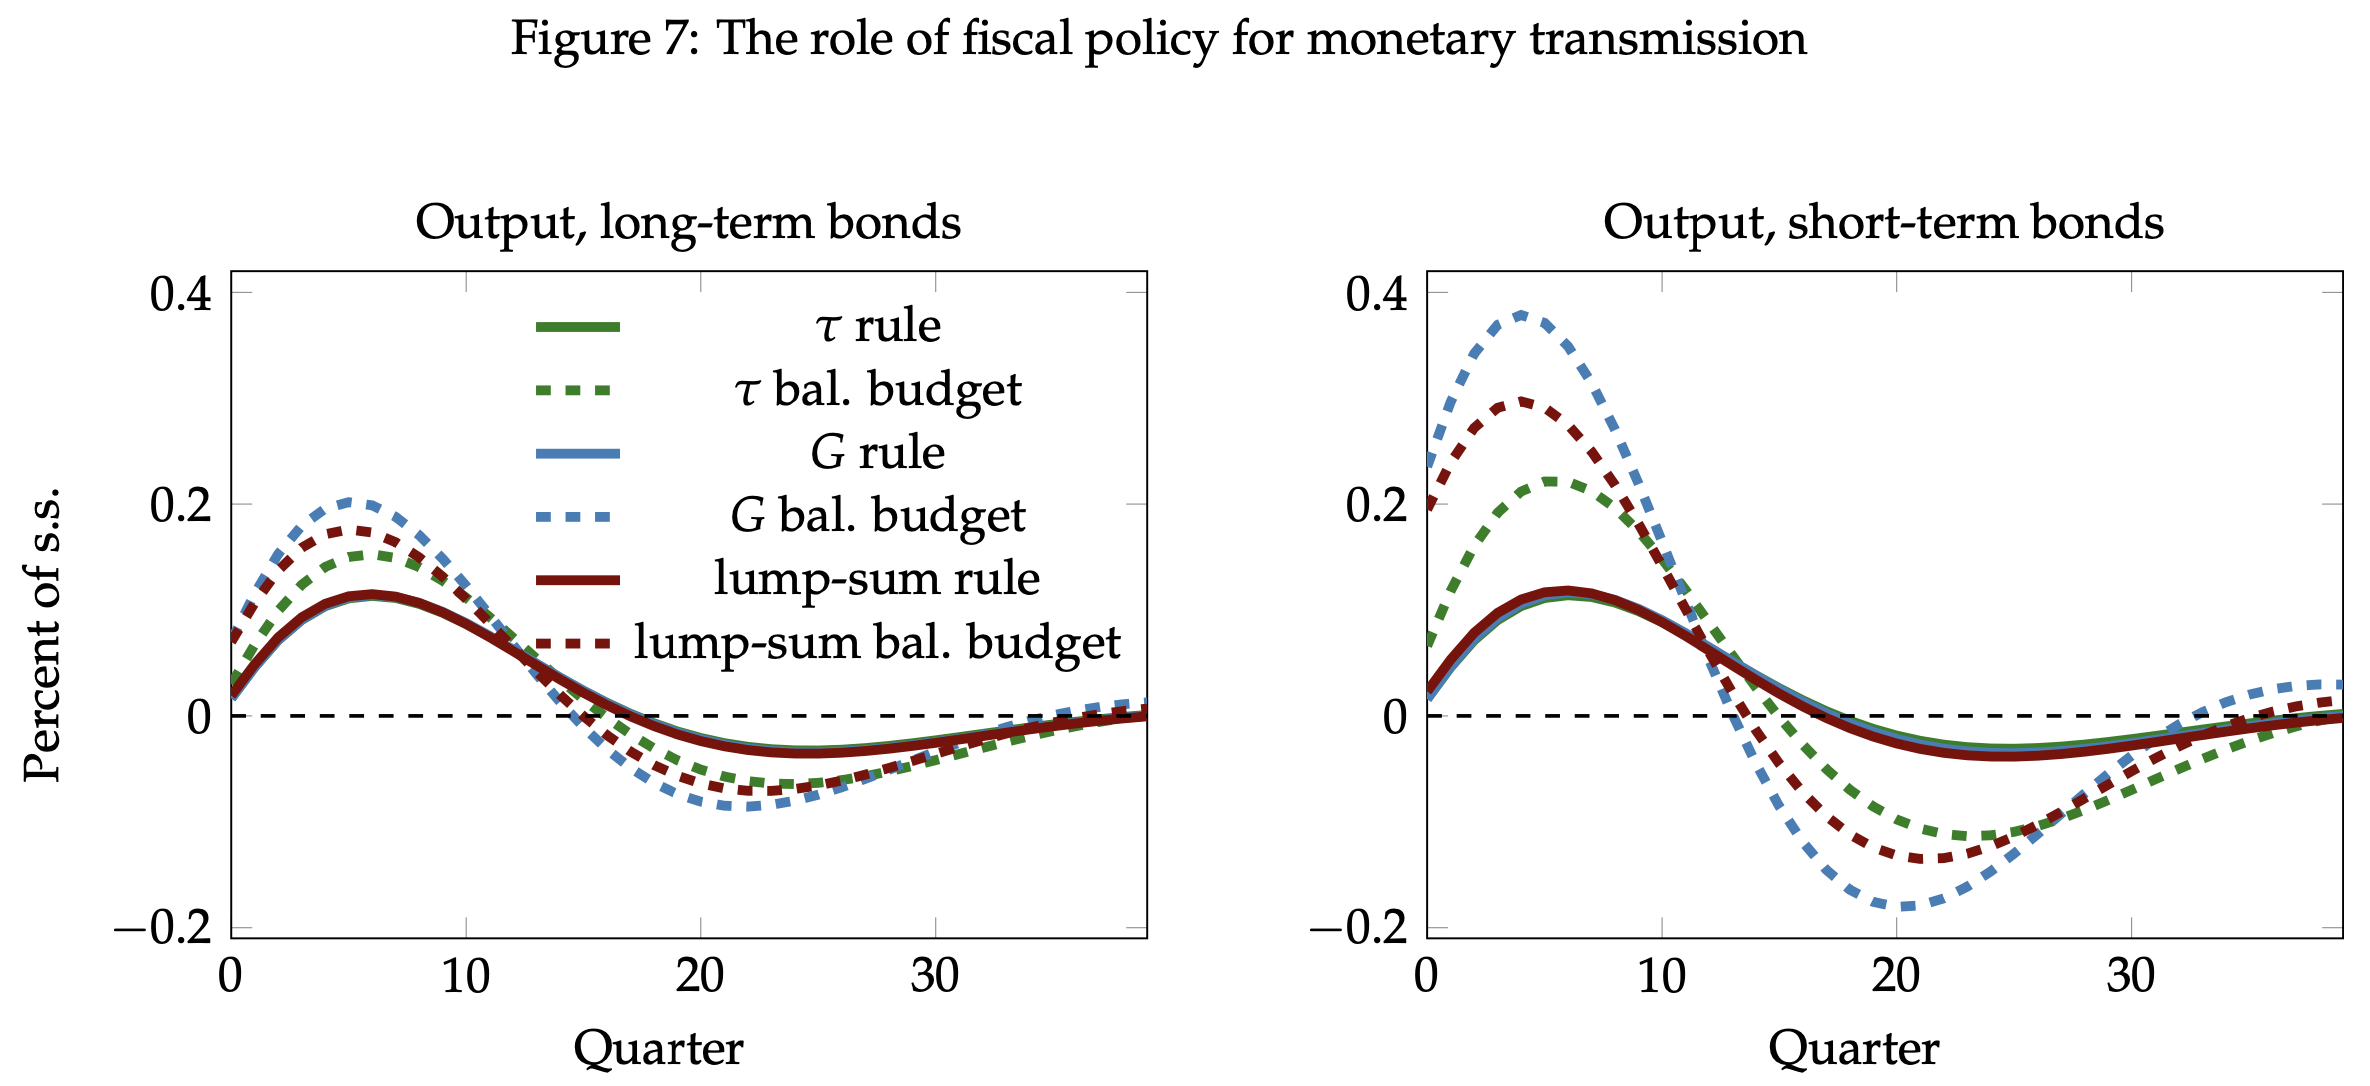
\includegraphics[scale=0.25]{figures/ARSFIG7.png}	
    \end{center}
\end{frame}

\begin{frame}
    \frametitle{Starting the Transmission Mechanism}
    \begin{center}
    	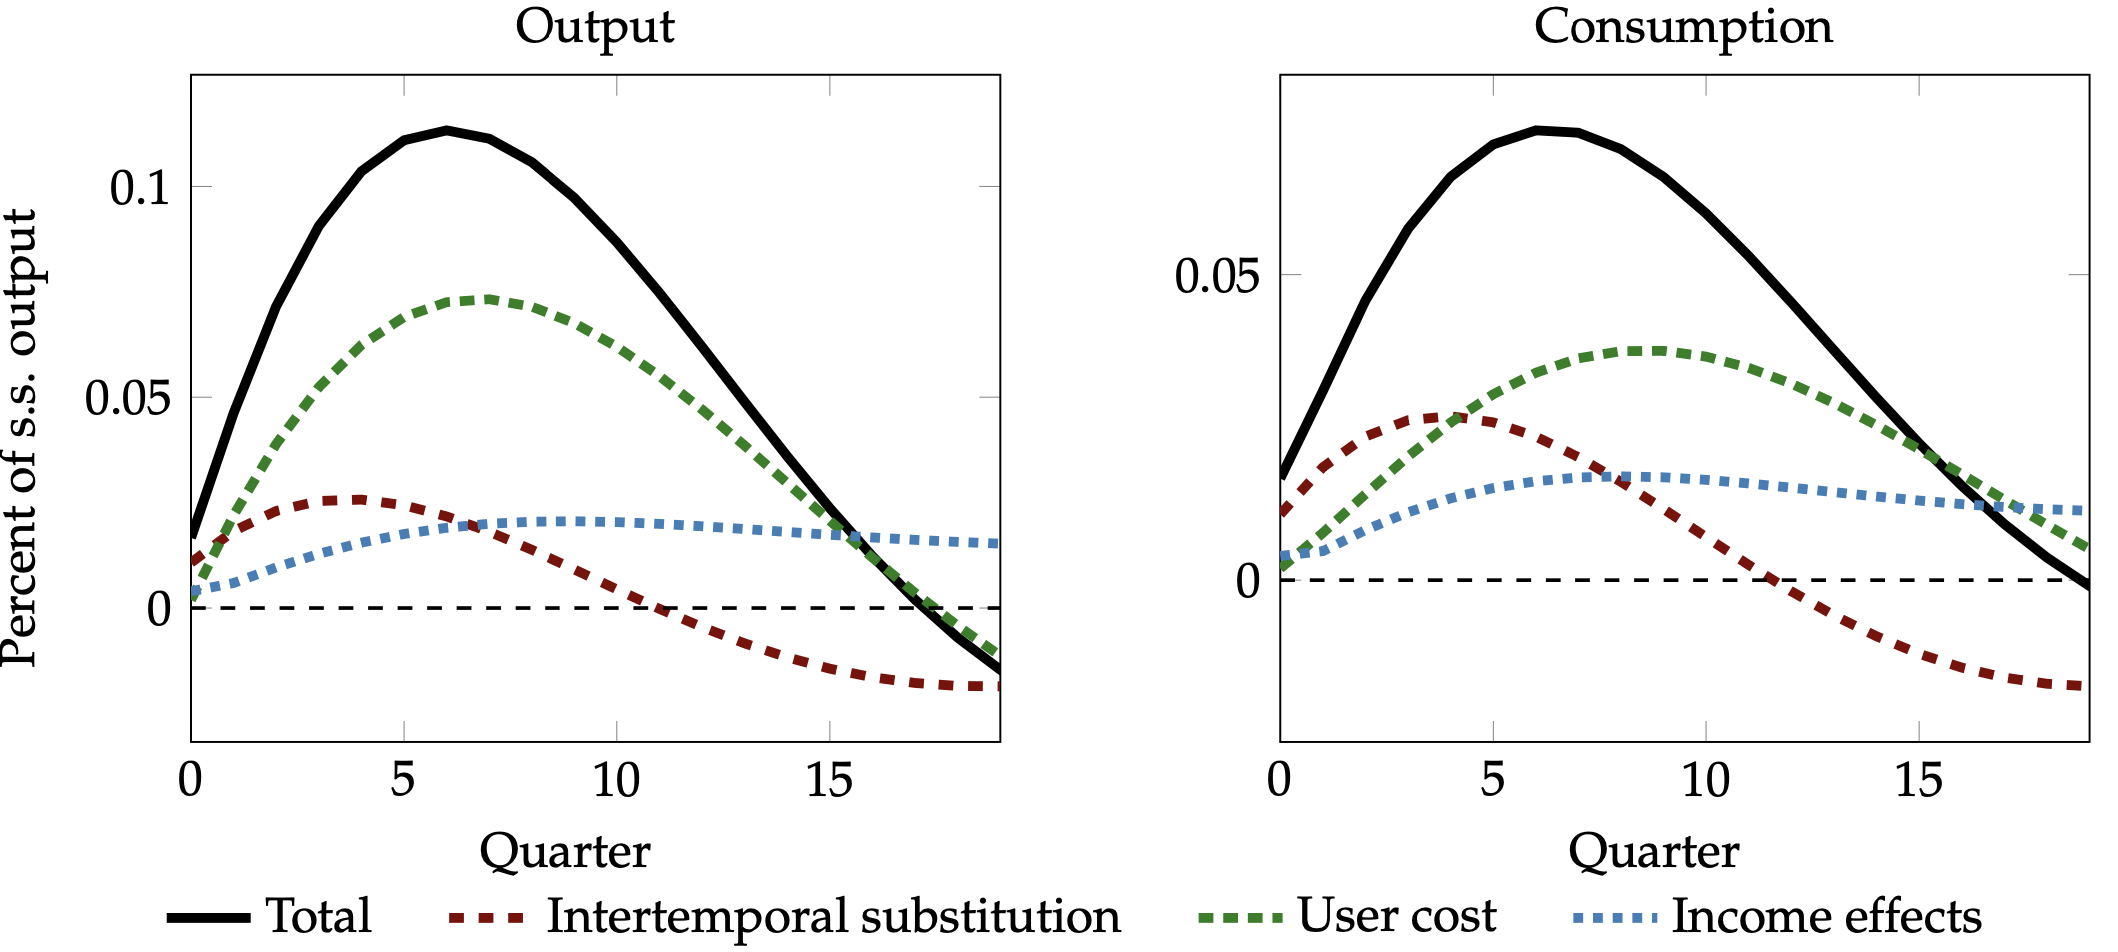
\includegraphics[scale=0.3]{figures/ARSFIG8.png}	
    \end{center}
\end{frame}


\begin{frame}
    \frametitle{Reassessing the Importance of Investment}
    \begin{center}
    	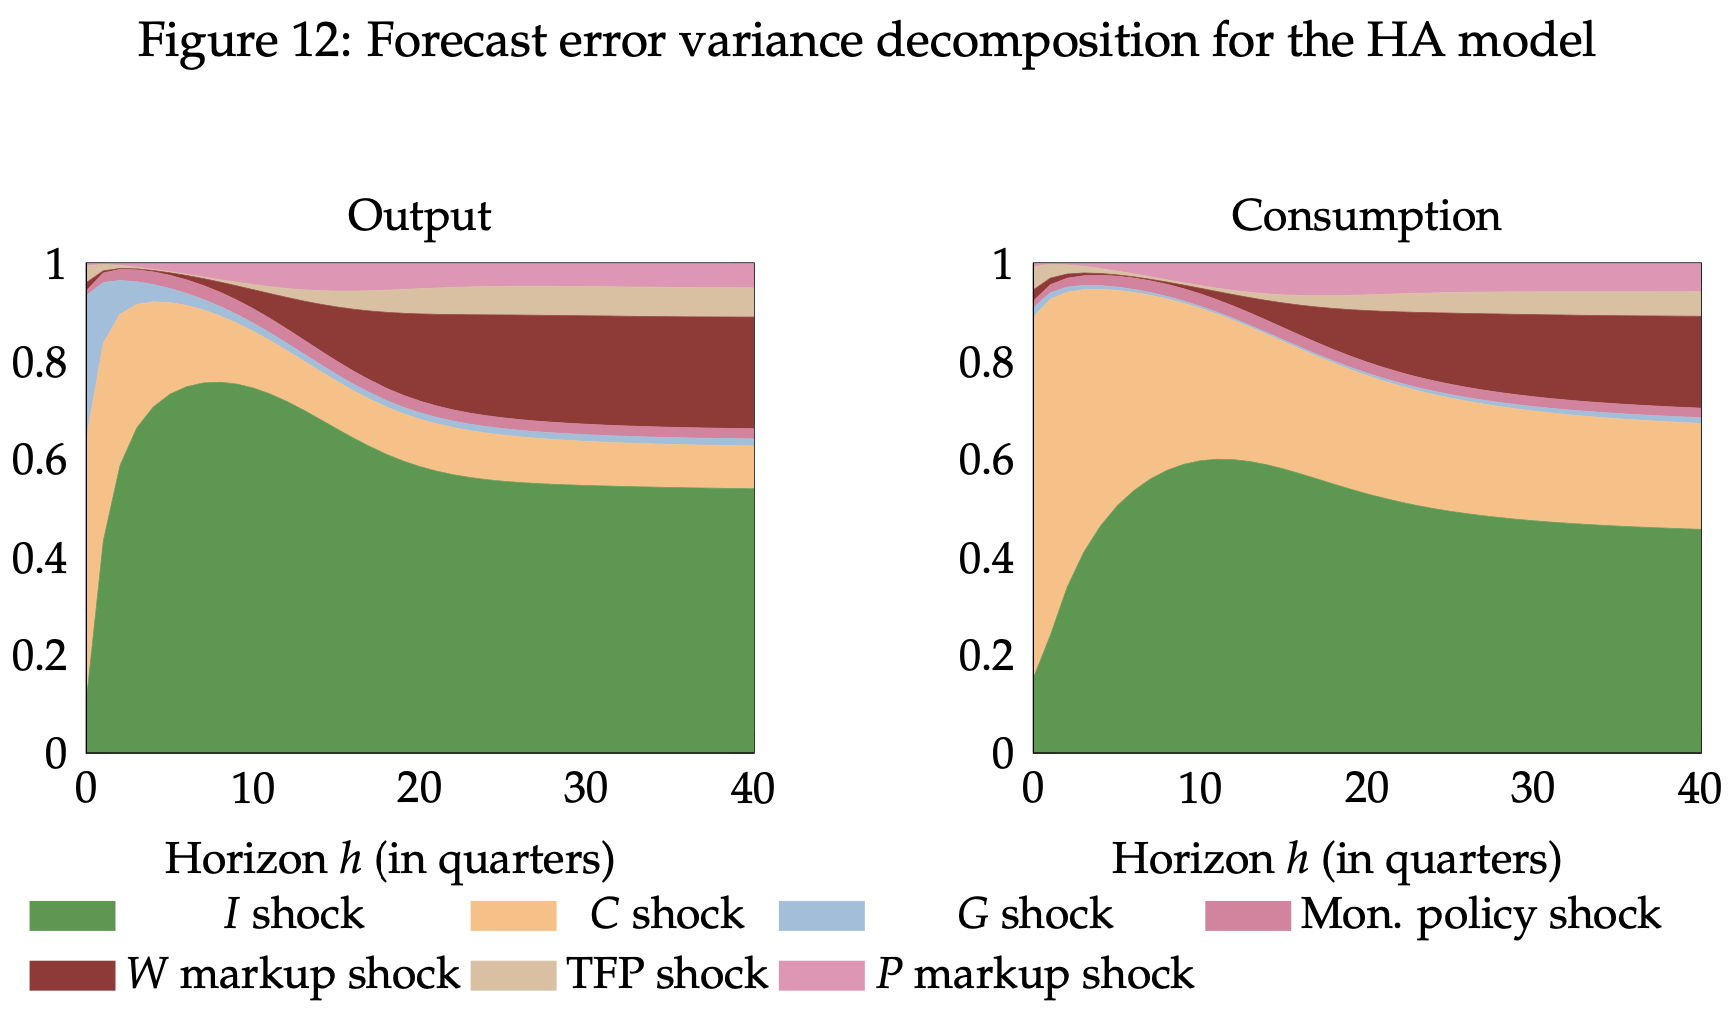
\includegraphics[scale=0.3]{figures/ARSFIG12.png}	
    \end{center}
\end{frame}



\end{document}